\newpage
\section{Background}
\label{sec:background}

This chapter presents a background discussion of deployment scenarios for data-parallel systems and the dominant architectures in the commercial space for such systems.
Saturn, as an implementation of a modern scalable vector ISA targeting deployment in specialized cores, fills an underexplored niche in the space of open-source data-parallel microarchitectures.
A comparison of Saturn's microarchitecture philosophy to alternative vector approaches is discussed.

\subsection{Data-parallel Workloads}

\begin{figure}[h]
  \centering
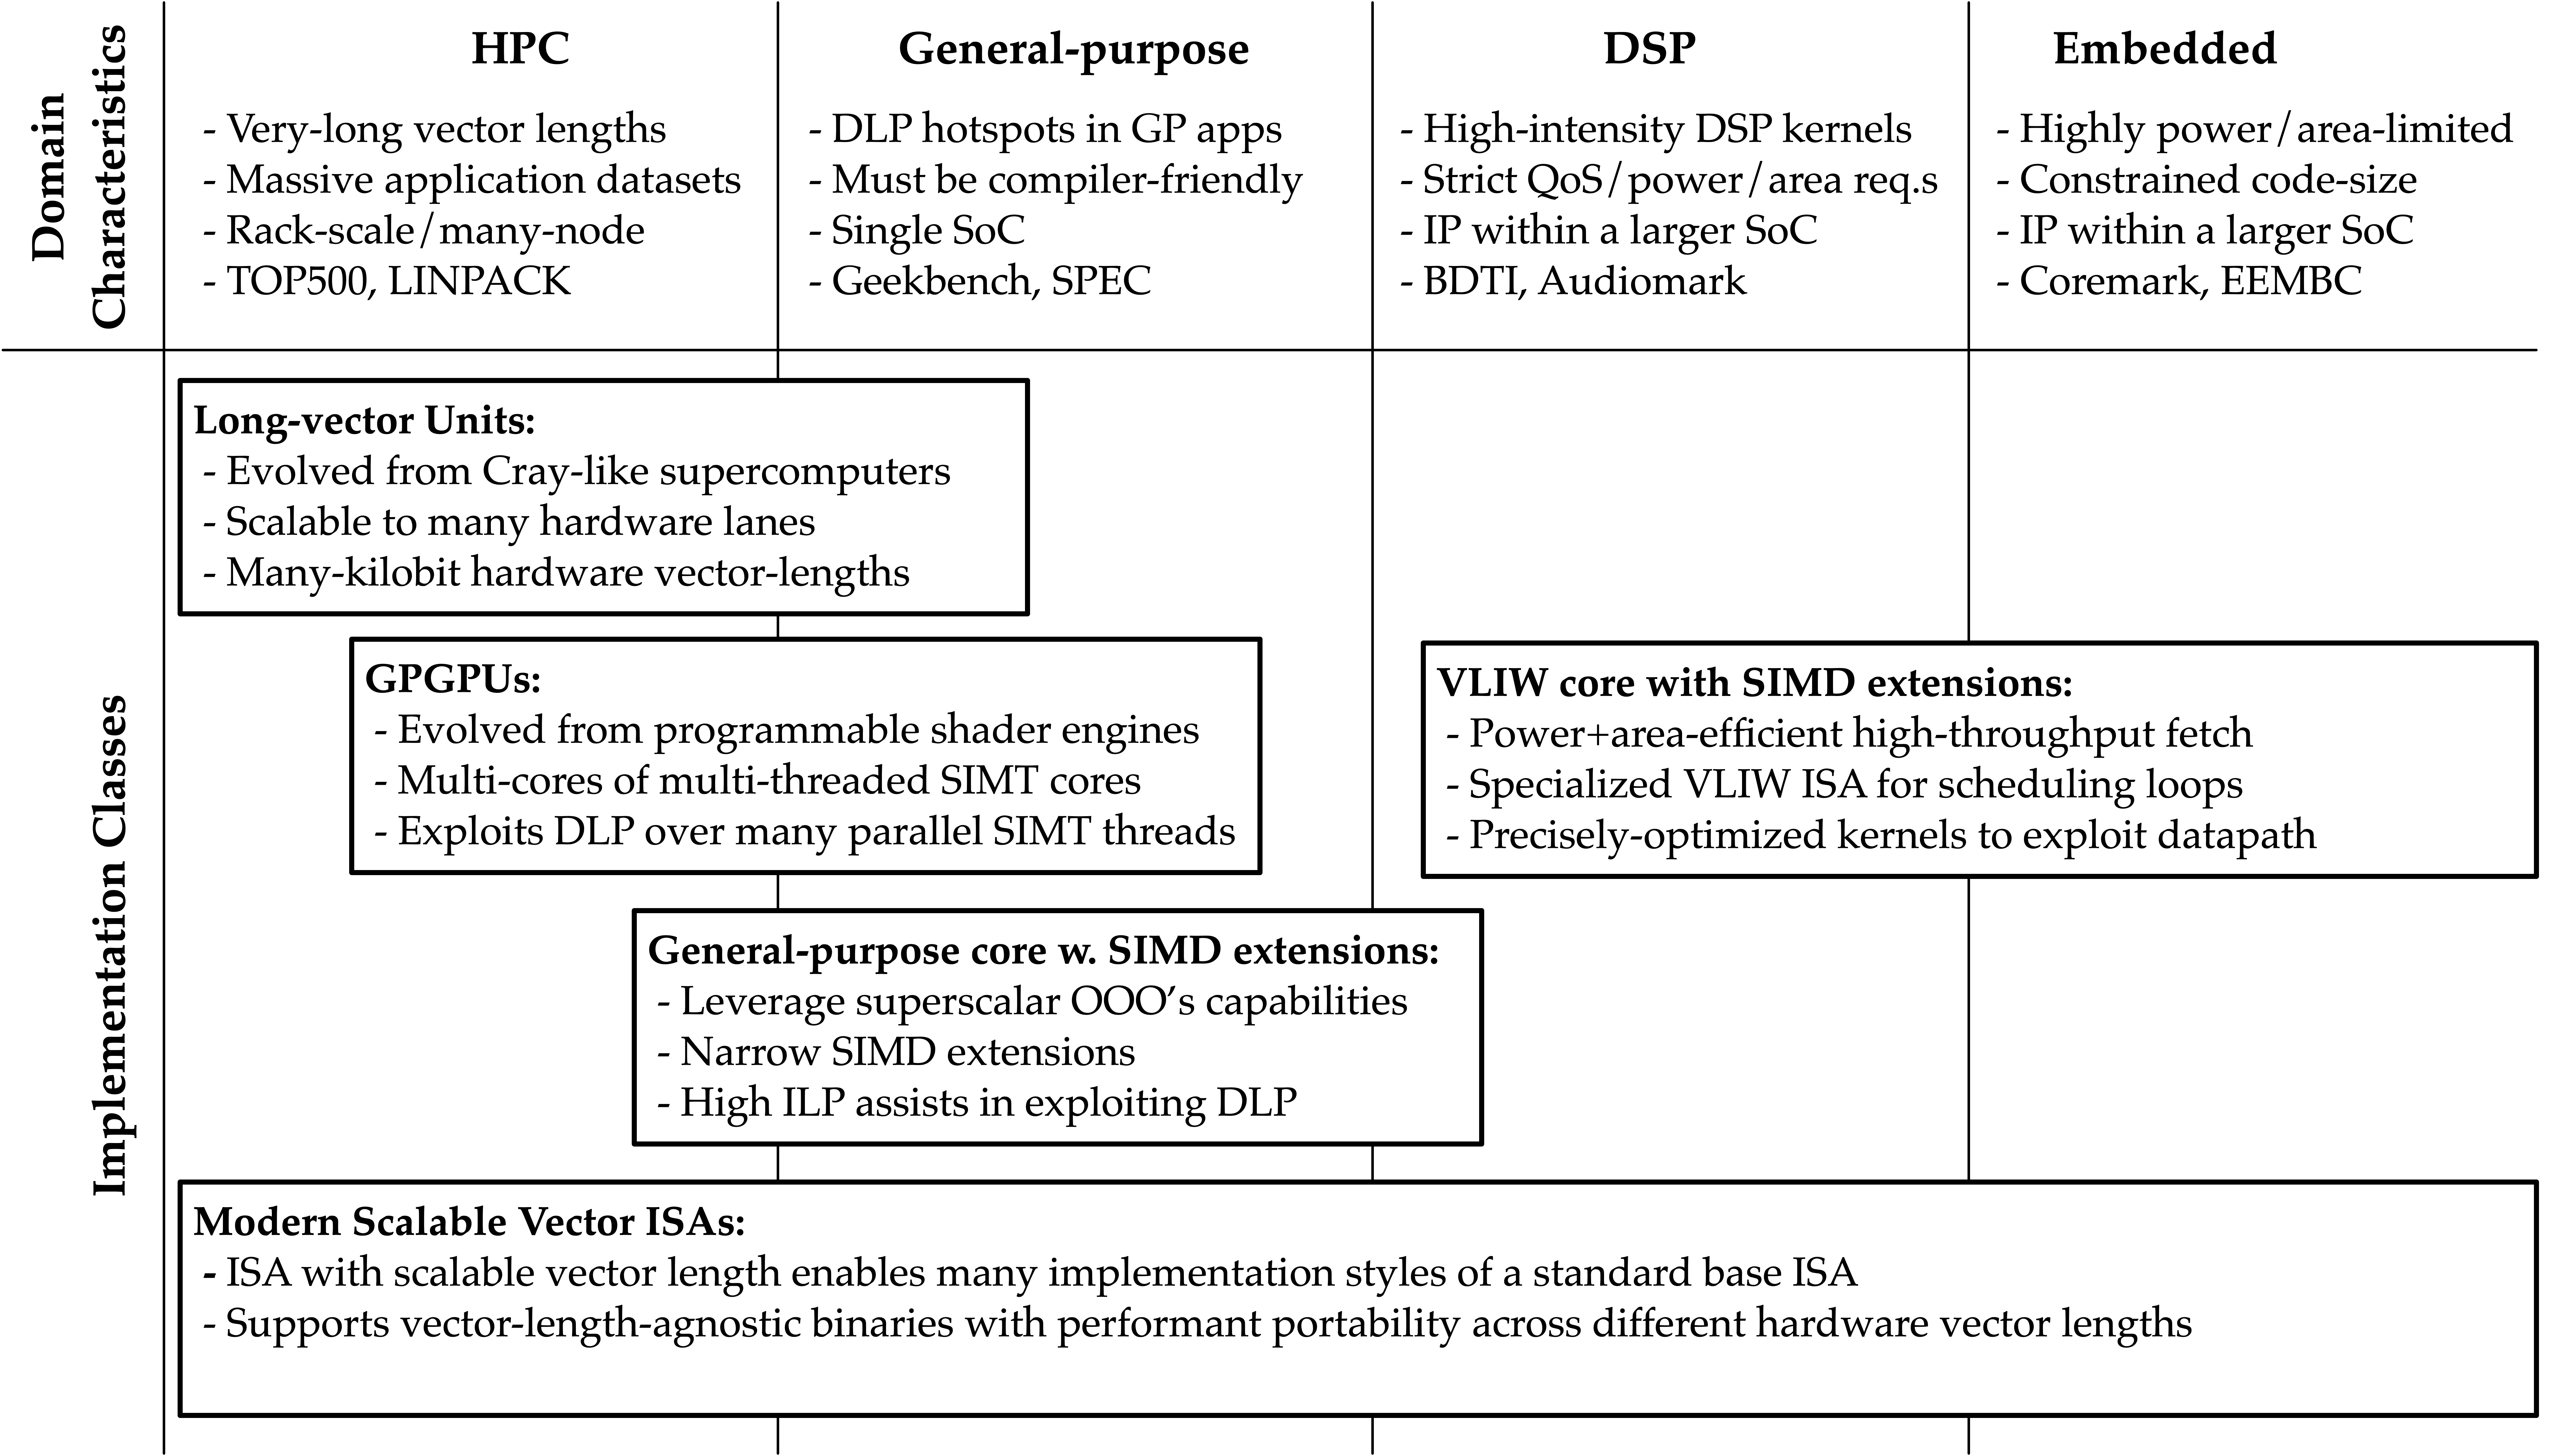
\includegraphics[width=\linewidth]{domains.png}
\caption{Taxonomy of data-parallel domains and their dominant architectures}
\label{fig:taxonomy}
\end{figure}

We broadly categorize the range of deployment scenarios and workloads for programmable data-parallel systems into four domains.
These categories are differentiated by power/area constraints and workload characteristics.
Figure \ref{fig:taxonomy} outlines the four deployment domains where DLP-enabled architectures are critical, and the salient architectural and microarchitectural archetypes that have come to dominate each domain.

\textbf{HPC, scientific computing, and ML training workloads} are typically characterized by very long application vector lengths, exhibiting a high degree of data-level parallelism.
Systems targeting these workloads are generally designed and deployed at datacenter scale, with available data-level-parallelism exploited across the many processors in a multi-node cluster.
While single-core efficiency and performance remain important for this domain, scalability towards multi-core, multi-node systems is of more critical concern.

\textbf{General-purpose server, desktop, and mobile workloads} intersperse data-level-parallel codes with sequential, control-flow heavy non-data-parallel blocks.
The implications of Amdahl's Law dictate the design of these systems; exploiting data-level parallelism must not come at the expense of single-thread performance or thread-level-parallelism.
Compared to the other domains, compiler and programmer-friendly ISAs are particularly important for these systems, as they must remain performant on the greatest diversity of workloads.

\textbf{Digital signal processing (DSP) and similar domain-specialized workloads} exploit fundamentally data-parallel algorithms.
These workloads are often offloaded in modern SoCs to specialized ``DSP cores" optimized towards power and area-efficient exploitation of data-level parallelism, with less consideration towards general-purpose performance.
``DSP cores" usually run optimized kernels written by programmers at a low level to maximize efficiency. 
Large SoCs typically integrate many such ``DSP cores" across various design points to provide optimized compute for different subsystems.

\textbf{Applications executing on embedded devices} face extreme constraints around power, area, and code size.
Exploiting data-level parallelism can be critical for these workloads as well, but might come as a secondary concern compared to power and area.
As these cores often provide a self-contained memory system, code and data size are more critical architectural considerations.

\subsection{Data-parallel Implementation Archetypes}

The requirements of the common data-parallel workload domains have induced the commercial space to converge towards several fundamental architectural and microarchitectural archetypes.

\subsubsection{Long-vector Implementations}

\textbf{Long-vector ISAs} and their \textbf{many-lane vector-unit} implementations trace their heritage most clearly to the early Cray-style vector units.
Modern incarnations of such systems primarily target the HPC and datacenter space, where long application vector lengths map cleanly into high-capacity vector register files.

Microarchitecturally, these implementations distribute the vector register file, functional units, and memory access ports across many vector lanes, with scalability towards many lanes being a key requirement.
A single core of such a vector unit might have upwards of 32 parallel vector lanes, with a hardware vector length of over 16384 bits.

Notably, a lane-oriented microarchitecture with distributed memory ports and a high-radix memory interconnect enables high performance on codes which require high address generation throughput.
Indexed loads and stores can leverage the distributed memory access ports to maintain high memory utilization, while register-register scatters and gathers can leverage a complex yet scalable cross-lane interconnect.

The NEC Aurora~\cite{nec_aurora} is a modern example of a commercial long-vector microarchitecture, while Hwacha~\cite{hwacha_manual}, Ara~\cite{ara2}, and Vitruvius~\cite{minervini_vitruvius_2023} are examples of academic long-vector implementations.

\subsubsection{SIMT GP-GPUs}

\textbf{GP-GPUs} execute a specialized \textbf{SIMT} ISA across a multi-core of multi-threaded processors.
GP-GPUs evolved from the need for increasingly programmable shader pipelines in graphics workloads.
Programming models for shaders developed into general-purpose SIMT frameworks like CUDA and OpenCL.
GPU implementations similarly became more general-purpose, eventually maturing into modern GP-GPU microarchitectures.

Notably, the multi-core SIMT archetype in GP-GPUs naturally adapts to a range of deployment domains.
By scaling the number of multi-threaded cores, GP-GPU microarchitectures can target integrated GPUs in general-purpose SoCs, graphics accelerator cards for desktop/consumer systems, as well as interconnected compute cards for datacenter-scale HPC systems.
The rise of GP-GPUs is a contributing factor to the decline of specialized long-vector microarchitectures for datacenter HPC systems.

In the commercial space, NVIDIA and AMD dominate the GP-GPU market.
Their HPC and datacenter products, while originally derived from consumer GPU architectures, have since diverged towards a more differentiated, yet still multi-core-SIMT microarchitecture.

Within the general-purpose mobile consumer space, AMD, Intel, Apple, Qualcomm, and Huawei all deploy embedded GP-GPU systems within their SoCs.
These vendors all provide developer SDKs for supporting general purpose applications on their GP-GPU microarchitectures.


\subsubsection{General-purpose ISAs with SIMD}

\textbf{General-purpose ISAs with SIMD extensions} enable exploiting data-level parallelism in a microarchitecture already optimized towards scalar IPC.
SIMD extensions evolved from subword-SIMD ISAs designed to pack a small fixed-length vector of sub-register-width elements within a single scalar register.
Subword-SIMD is a cheap way to integrate limited forms of data-parallel compute, particularly for multimedia applications, into a general-purpose processor, without requiring substantial redesign of complex microarchitectural components.
Modern SIMD ISAs have generally moved beyond subword-SIMD (except in the embedded space) towards wider SIMD registers.

Microarchitectures of general-purpose cores perform instruction scheduling of SIMD instructions using similar mechanisms as they do for scalar instructions.
Existing features like superscalar issue, out-of-order execution, and register renaming can be reused to maintain high instruction throughput into the SIMD functional units.
This paradigm has largely held even in modern general-purpose-SIMD cores, which feature much wider SIMD registers than scalar registers for improved performance on data-parallel workloads.

Practically all widely deployed commercial general-purpose cores ship with SIMD extensions.
Intel and AMD out-of-order cores support some form of the SSE or AVX extensions~\cite{intel_avx}, while ARM's A-profile~\cite{armv8a} architecture requires NEON.
 
\subsubsection{VLIW ISAs with SIMD}

\textbf{VLIW ISAs with SIMD extensions} have traditionally dominated the space of DSP and similar domain-specialized cores, as well as embedded cores.
For these deployment scenarios, power and area constraints preclude the deployment of costly microarchitectural features towards high instruction throughput in a general-purpose ISA, such as speculative execution and register renaming.
The structure of DSP kernels presents a good fit for the VLIW paradigm, since regular loops, rather than branch-dense control code, are easier to optimize on a VLIW microarchitecture.

Furthermore, DSP applications often require more regularly behaved memory systems to achieve strict QoS requirements, leading to DSP cores often integrating low-or-fixed-latency software-managed scratchpad memories, rather than caches with dynamic, unpredictable behavior.
Applications and microarchitectures which prefer statically predictable memory systems are especially well-suited for VLIW ISAs.

However, VLIW-based ISAs are notoriously difficult to program compared to general-purpose ISAs or vector ISAs.
Performant VLIW code can also suffer from issues such as large static code size due to the need for extensive static scheduling and software-pipelined loops.
Nonetheless, specialized VLIW ISAs provide a microarchitecturally simple and efficient programmer-visible mechanism for maintaining high instruction throughput into SIMD functional units.

Cadence, Synopsys, CEVA, and Qualcomm all ship commercial VLIW DSPs with SIMD extensions.
Cadence, Synopsys, and CEVA cores are IP products typically integrated into a customer's SoC as an embedded core, while Qualcomm's Hexagon DSP Cores are integrated throughout their SoC line to provide DSP compute.

\subsubsection{Scalable Vector ISAs}

In contrast to the above patterns, modern \textbf{scalable vector ISAs} aspire to provide a common unified ISA that can support a range of microarchitectural implementation styles, supporting long-vector Cray-like machines, general-purpose out-of-order machines with vector extensions, specialized DSP cores with vector extensions, as well as ultra-compact embedded vector units.
The dominant examples of such ISAs include ARM's proprietary SVE~\cite{arm_sve} and MVE~\cite{arm_mve} extensions, as well as the open RISC-V Vector extension~\cite{vector_extension}.

Existing academic implementations of RVV have broadly targeted the HPC and general-purpose deployment scenarios with long-vector or out-of-order-core-integrated microarchitectures.
Compared to most prior academic implementations, Saturn targets DSP and domain-specialized cores, and represents a class of designs we call *``short-vector"*.

Existing open-source ``short-vector" implementations like Spatz~\cite{spatz}, Vicuna~\cite{vicuna}, and RISCV-2~\cite{patsidis_risc-v2_2020} require either register-renaming or constricted memory systems.
RISCV2 requires register-renaming, while Spatz and Vicuna assume a low-latency memory system.
Vicuna further requires a global stall to adapt to variable memory latencies.
Unlike these designs, Saturn demonstrates that a ``short-vector" design can achieve high performance and efficiency without any architectural or microarchitectural sacrifices.

\subsection{The RISC-V Vector ISA}

The RISC-V Vector ISA is the standard extension in RISC-V for exploiting data-level parallelism.
A full discussion of the ISA design can be found in its specification~\cite{vector_extension}.
This section highlights several properties of RVV that pose notable challenges to implementation or distinguish it from other vector ISAs.


\subsubsection{Dynamic Vector Type and Length}

Stripmine loops in RVV use \texttt{vset} instructions to dynamically adjust vector configuration state in the body of the loops.
These instructions set the dynamic \texttt{vl} vector length register in addition to the \texttt{vtype} register, which sets the element width, register grouping, and mask/tail agnosticity for subsequent operations.

A naive implementation of RVV might treat the \texttt{vtype} as a single system-wide register, owing to its effect on the behavior of many components of the vector datapath.
However, such an approach would substantially degrade performance, as \texttt{vset} is used in the inner loops of vector kernels to effect stripmining or to enable mixed-precision kernels.

As a result, performant implementations must maintain copies of the \texttt{vtype} and \texttt{vl} registers, instead of maintaining a single global status.
Since neither \texttt{vtype} nor \texttt{vl} require many bits to encode, this state can be renamed into a control bundle that propagates alongside each vector instruction in the datapath.

Furthermore, since \texttt{vtype} and \texttt{vl} affect the generation of precise faults by vector memory instructions, it is insufficient to update these registers only at commit, since precise faults must be generated ahead of commit.
Doing so would introduce an interlock between a \texttt{vset} and a subsequent vector memory operation, which must stall until the \texttt{vset} commits before using the updated \texttt{vtype}/\texttt{vl} to check for precise faults.
Instead, performant scalar core implementations should bypass updates of \texttt{vtype} and \texttt{vset} to an early stage in the pipeline.


\subsubsection{Memory Disambiguation}

RVV mandates that vector memory operations appear to execute in instruction order with respect to \textbf{all} other instructions on the same hart, including scalar memory instructions.
While an alternative ISA design may have relaxed this ordering requirement, such an approach would necessitate costly and precise programmer-inserted fences to enforce scalar-vector memory ordering.

This requirement for scalar-vector memory disambiguation poses a challenge to decoupled post-commit vector unit implementations, in which vector loads and stores might run behind scalar loads and stores.
Stalling scalar loads and stores until the vector loads and stores drain could have costly implications on kernels which naturally would benefit from overlapping scalar and vector memory operations.
For instance, in an input-stationary matrix multiplication, the inner loop streams across scalar loads of an input tile and vector loads and stores of the output.
This kernel would naturally require efficient scalar-vector memory disambiguation.

Performant implementations should allow concurrent execution of scalar and vector memory operations by performing precise early-stage memory disambiguation of vector memory accesses.


\subsubsection{Precise Faults}

RVV mandates precise faults for vector memory operations.
Faulting vector loads and stores must execute up until the element which causes the fault, report the element index that generated the fault, and block commit of any younger scalar or vector instructions.
This implies that implementations must check for precise faults ahead of commit.

However, offloading address generation entirely ahead of-commit would have significant negative performance consequences, as this would stall unrelated scalar instructions even in the common case where instructions do not fault.
Performant implementations should expediently commit vector memory instructions in the common case where they do not fault, and only interlock the scalar core in the uncommon case where a fault is present.


\subsubsection{Vector Register Grouping}

The \texttt{LMUL} (length multiplier) register grouping field of \texttt{vtype} enables grouping consecutive vector registers into a single longer vector register.
In addition to enabling mixed-precision operations, this feature allows kernels that do not induce vector register pressure to access an effectively longer hardware vector length.
Generally, performance programmers for RISC-V will use this feature to reduce the dynamic instruction count of their loops and potentially improve the utilization of hardware compute resources.
For example, vector \texttt{memcpy} induces no register pressure and can trivially set a high \texttt{LMUL} to reduce dynamic instruction count.
Since higher \texttt{LMUL} settings will unroll instructions in hardware, \texttt{LMUL} also reduces static code size byreducing the need for unrolling loops in in software.

Thus, implementations should not penalize code which uses high \texttt{LMUL} to reduce instruction fetch pressure.
The general intuition around vector code should be to use the highest \texttt{LMUL} setting while avoiding register spills.
Implementations should should strive to support this intuition.

One tempting approach to implementing register grouping behavior would be to crack \texttt{LMUL > 1} instructions early in the pipeline and implement the backend instruction scheduling around \texttt{LMUL = 1}.
While this strategy is straightforward to implement as it simplifies the instruction scheduling, it may cause performance issues due to pressure on datapath scheduling resources from the many micro-ops generated by cracked high-\texttt{LMUL} instructions.
Alternatively, the addition of queueing resources to reduce this pressure would add significant area and power overhead.


\subsubsection{Segmented Memory Instructions}

Segmented memory instructions enable a ``transpose" of an ``array-of-structs" data representation in memory into a ``struct-of-arrays" in consecutive vector registers.
Such instructions, while very complex behaviorally, are fundamental to many algorithms and datatypes.
For instance, complex numbers and image pixel data are conventionally stored in memory as ``arrays-of-structs".

The instructions are critical for repacking data in memory into element-wise format for vector instructions.
Compared to other vector or SIMD ISAs, RVV provides few facilities for register-register repacking, instead relying on segmented memory instructions to perform ``on-the-fly`` repacking between memory and registers.

Given the importance of these instructions, performant RVV implementations should not impose an excess performance overhead from their execution.
Vector codes which use these memory operations should perform no worse than the equivalent code which explicitly transforms the data over many vector instructions.

\newpage
\subsection{Short-Vector Execution}

Saturn's instruction scheduling mechanism differentiates it from the relevant comparable archetypes for data-parallel microarchitectures.
Fundamentally, Saturn relies on efficient dynamic scheduling of short-chime short-vectors, without relying on costly register renaming.
When \texttt{LMUL} is short (1 or 2), vector chimes may be only 2-4 cycles long, requiring higher throughput scheduling than a long-chime machine.

\begin{figure}[h]
  \centering
  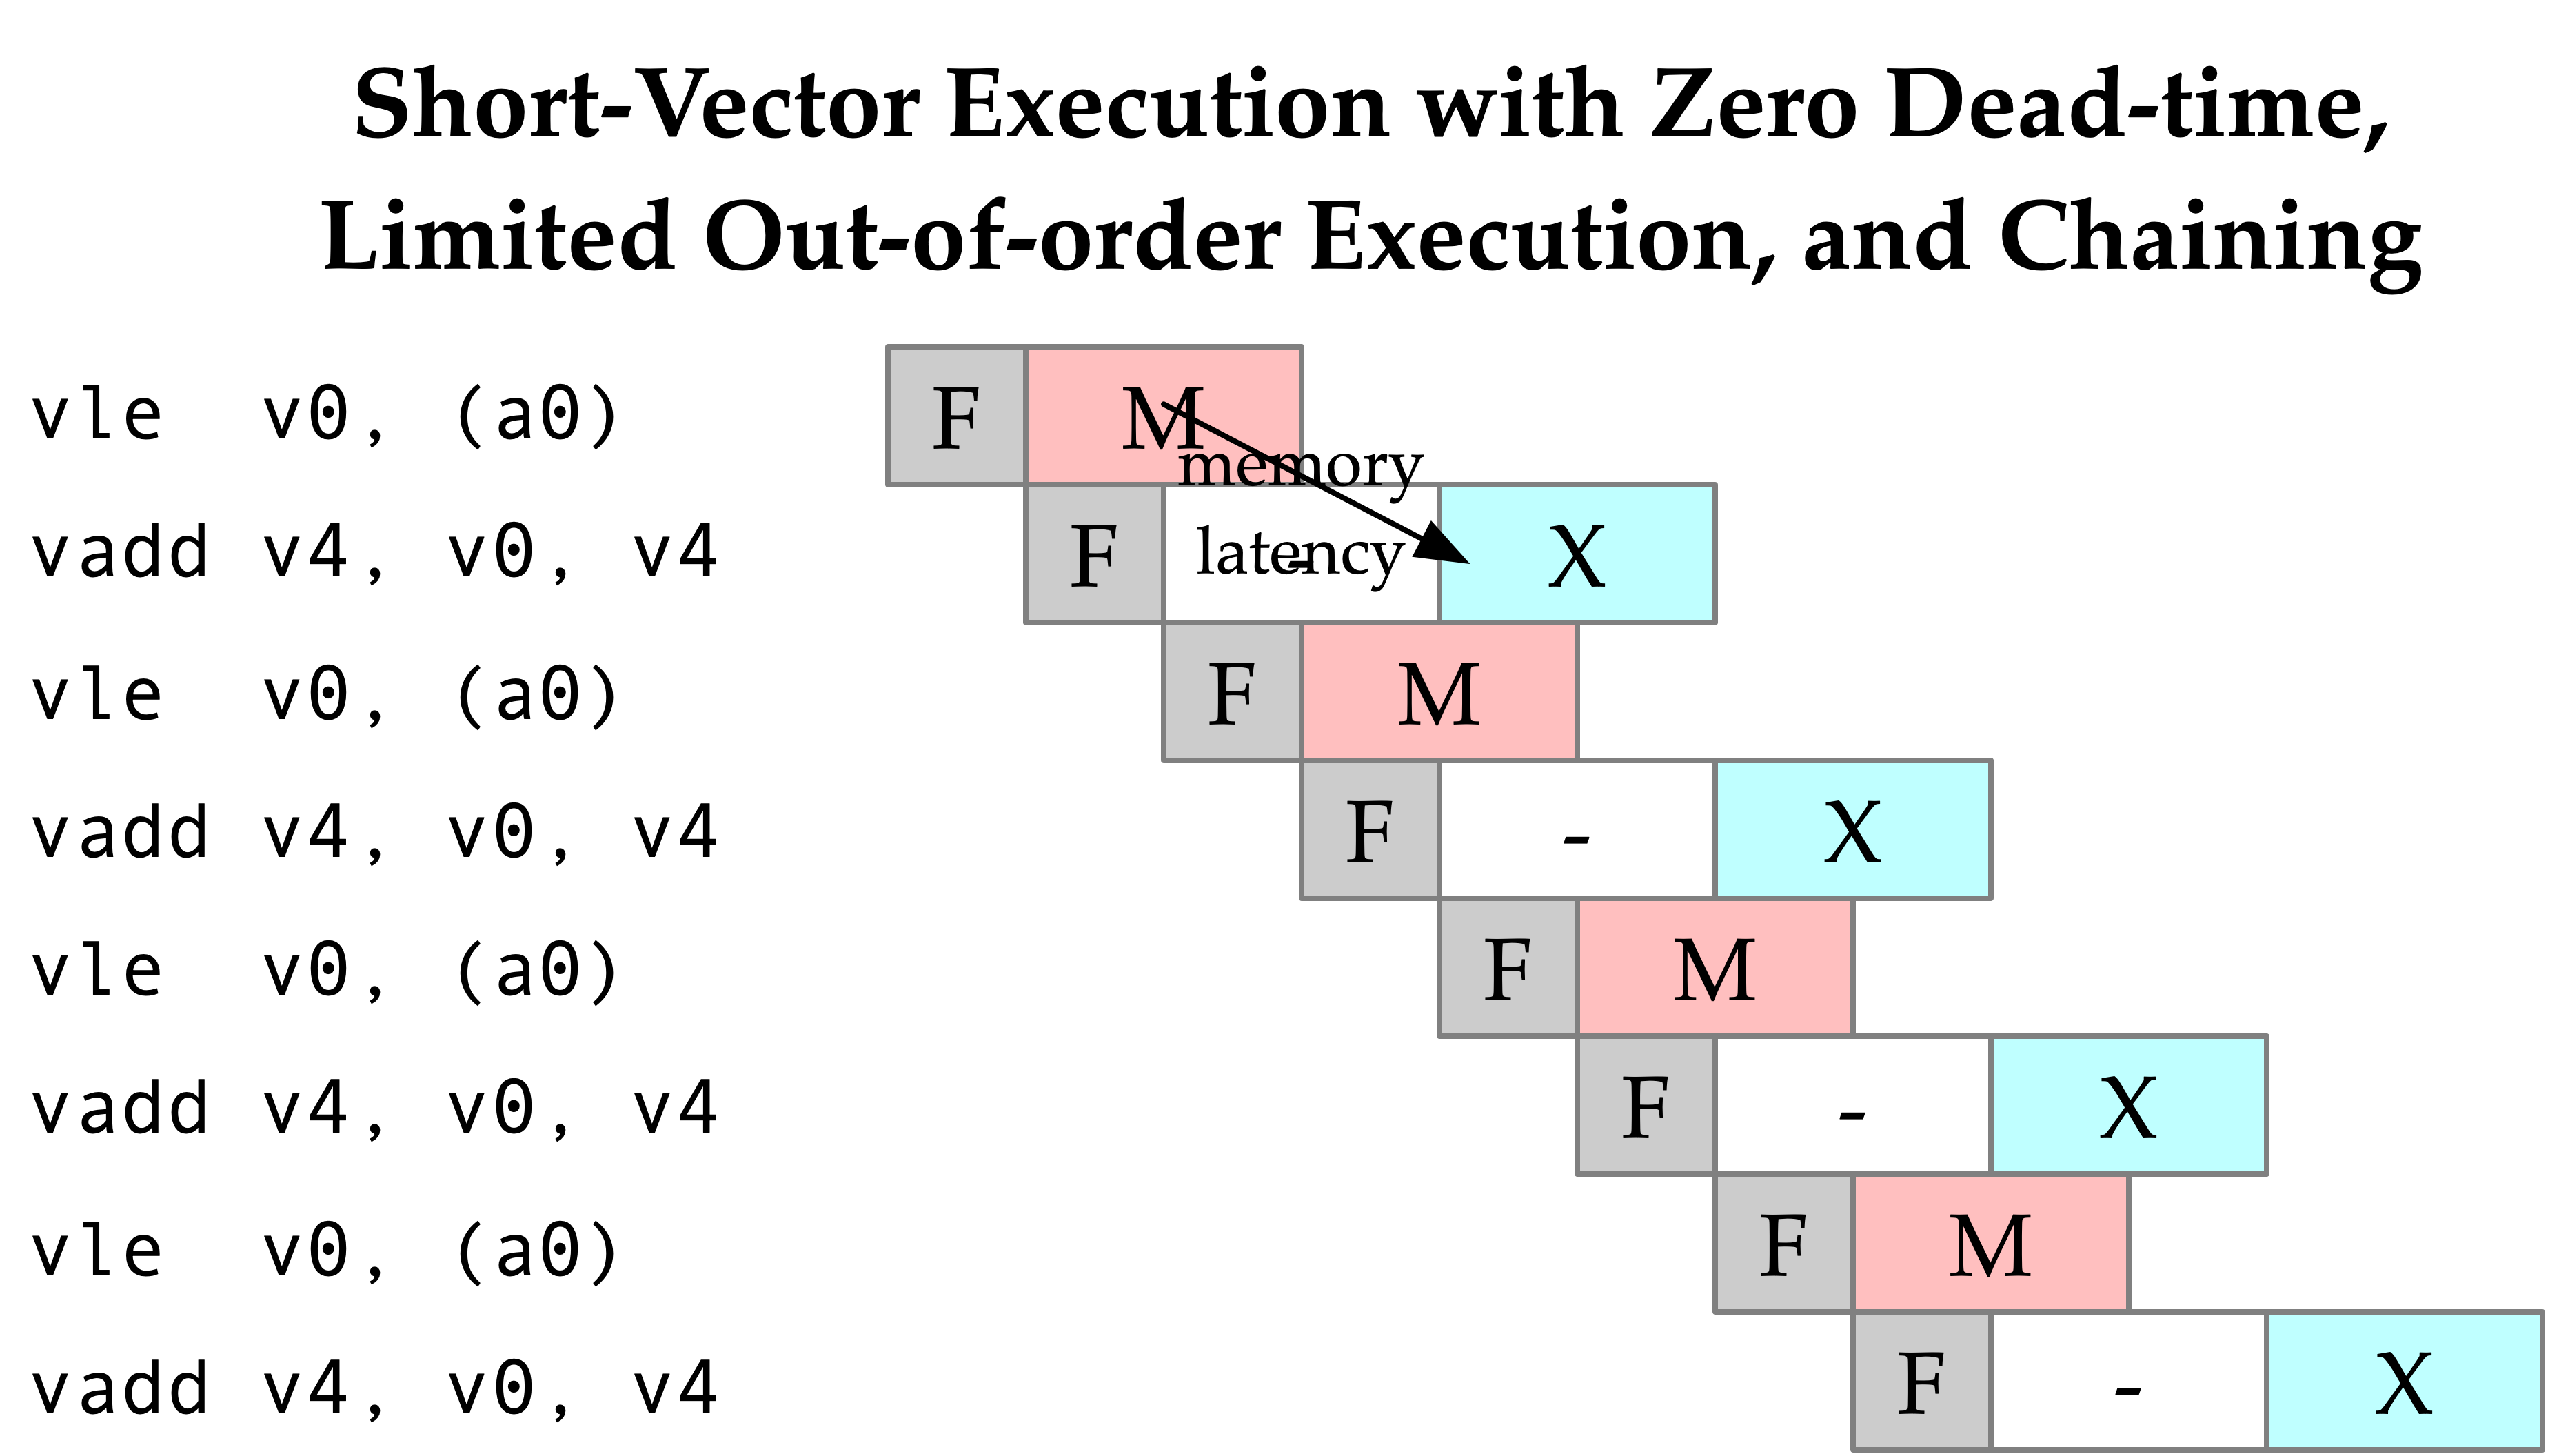
\includegraphics[scale=0.46]{short-vectors.png}
  \caption{Pipeline diagram of instruction execution with short vector lengths, zero dead time, limited out-of-order execution, and chaining. Instructions in the X and M pipelines can execute out-of-order w.r.t. each other.}
  \label{fig:short}
\end{figure}

Figure \ref{fig:short} depicts a simplified pipeline visualization of a short vector loop, consisting of a load and dependent arithmetic instruction, executing on a simplified Saturn-like short-vector datapath.
In this example, each vector chime is 2 cycles.


A short-vector machine should fully saturate both the arithmetic and memory pipelines with such short vector lengths and chimes.
Instruction throughput requirements are moderate, but can still be fulfilled with a modest superscalar in-order scalar core.
Notably, some degree of out-of-order execution, beyond just chaining, is necessary to enable saturating both the memory and arithmetic pipelines.

\begin{figure}[h]
  \centering
  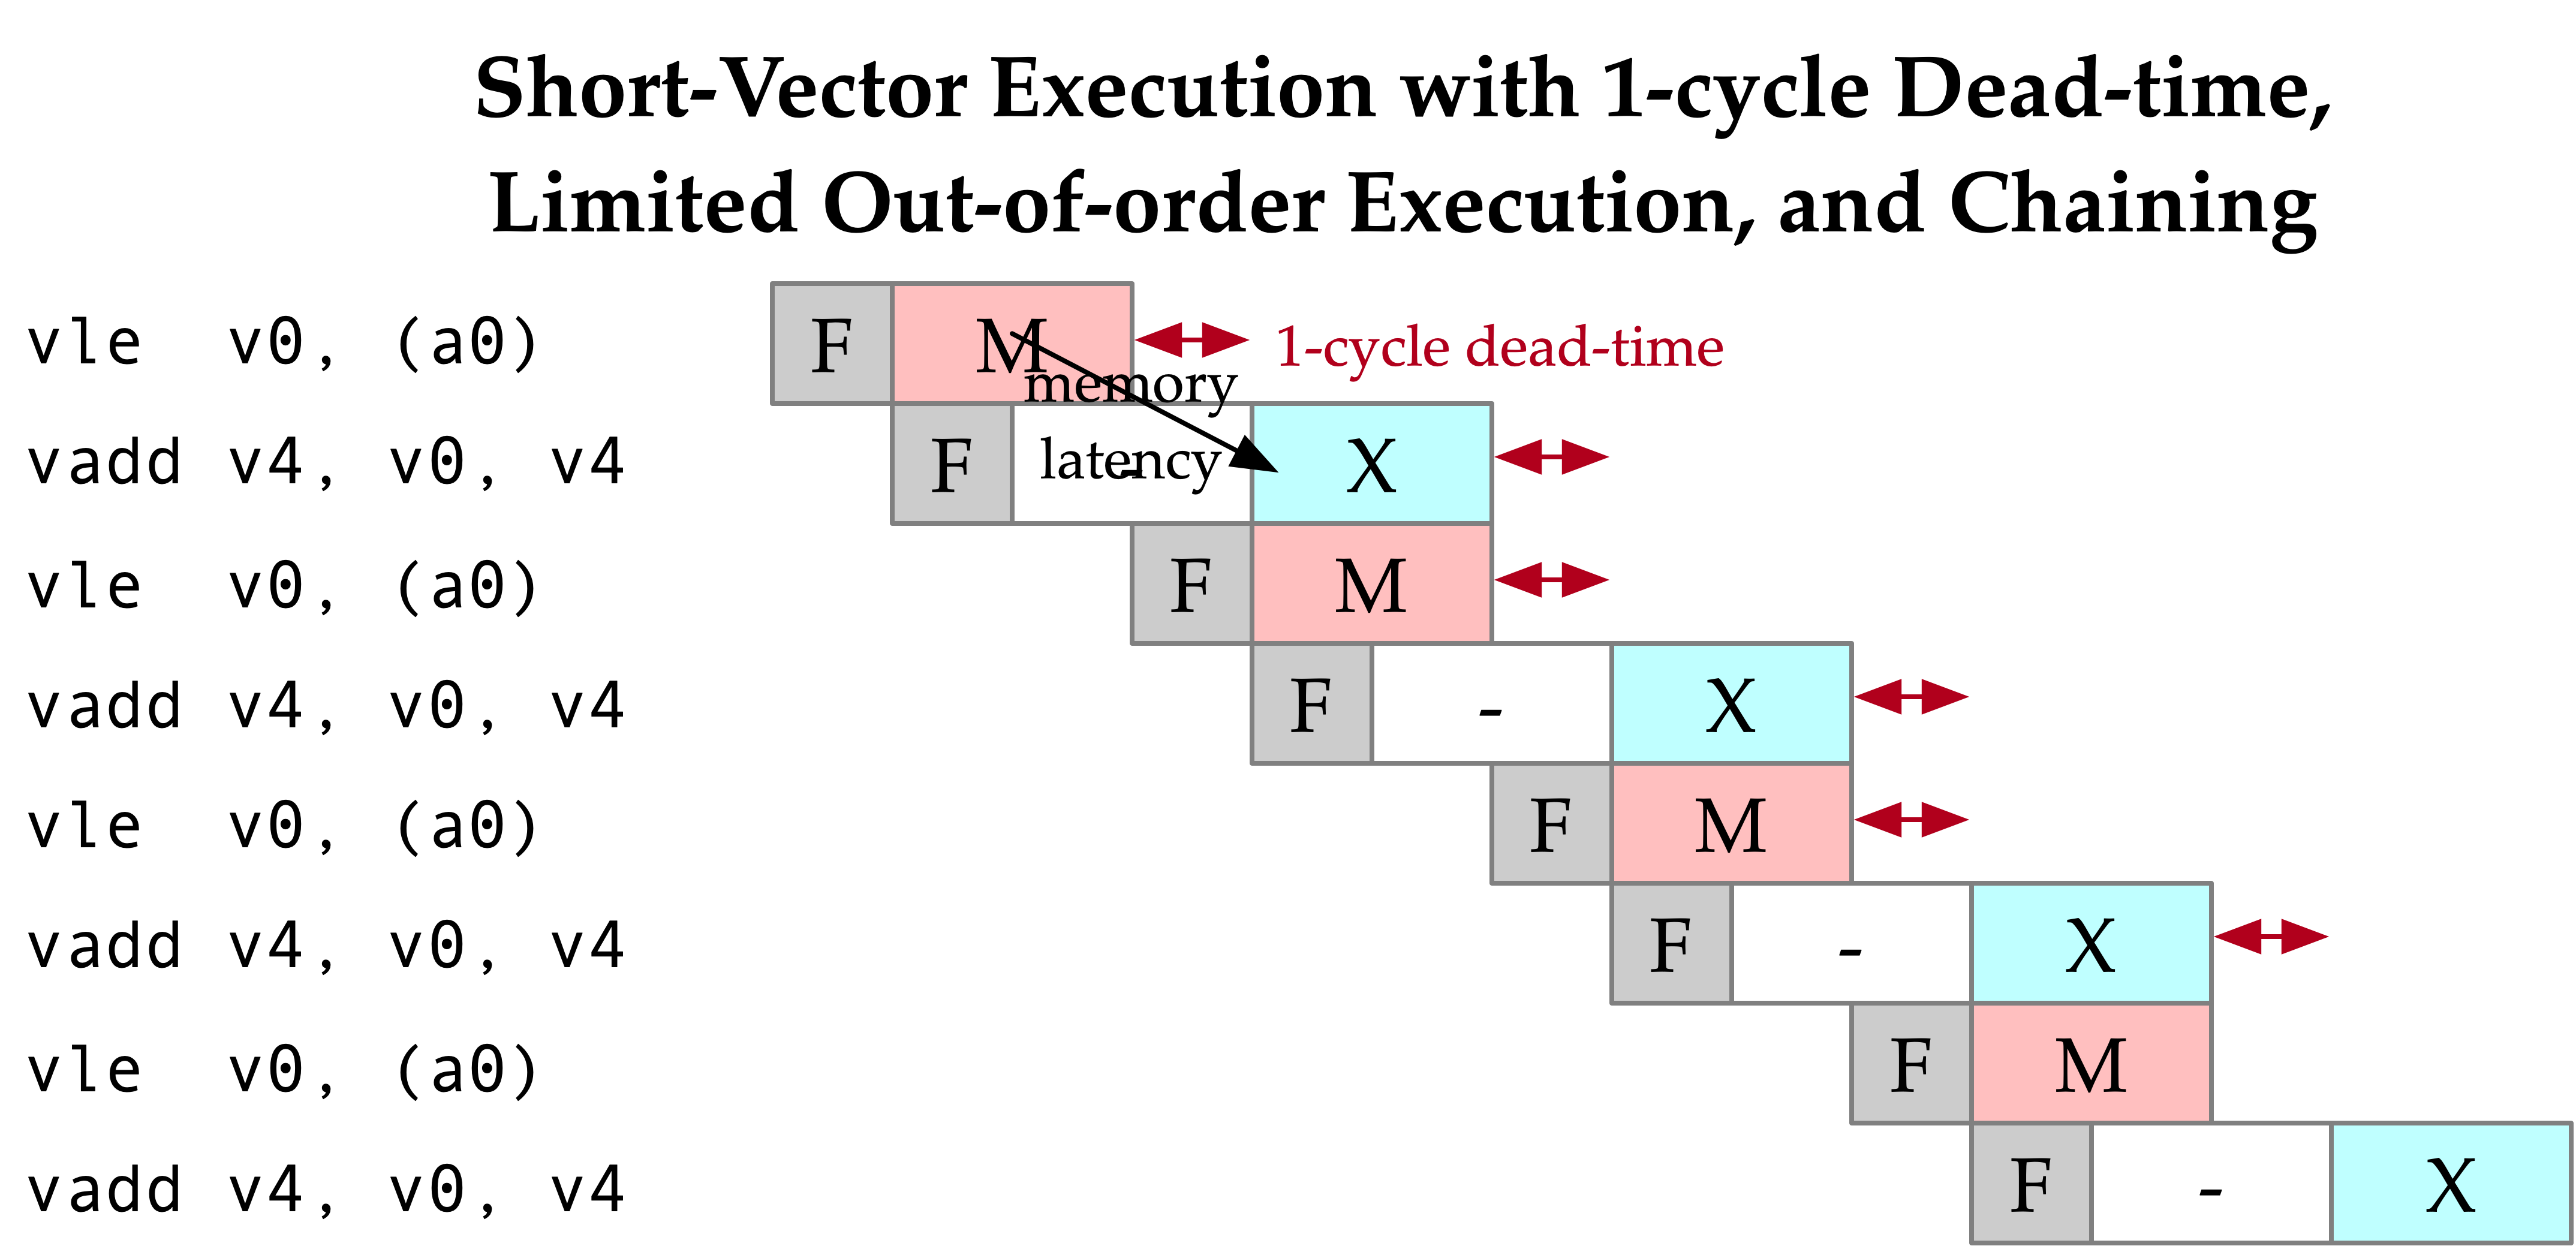
\includegraphics[scale=0.45]{short-vectors-dead.png}
  \caption{Pipeline diagram of instruction execution with short vector lengths, 1-cycle dead time, limited out-of-order execution, and chaining. Instructions in the X and M pipelines can execute out-of-order w.r.t. each other.}
  \label{fig:short-dead}
\end{figure}



Figure \ref{fig:short-dead} highlights the importance of zero dead time for short-vector microarchitectures.
Unlike in Figure \ref{fig:short}, the machine in this example has 1-cycle dead time for each functional unit, perhaps due to an inefficiency in freeing structural resources as instructions are sequenced.
A single cycle of dead time in a short-chime machine substantially degrades the utilizations of the datapaths, as the dead time cannot be amortized. 


\begin{figure}[h]
  \centering
  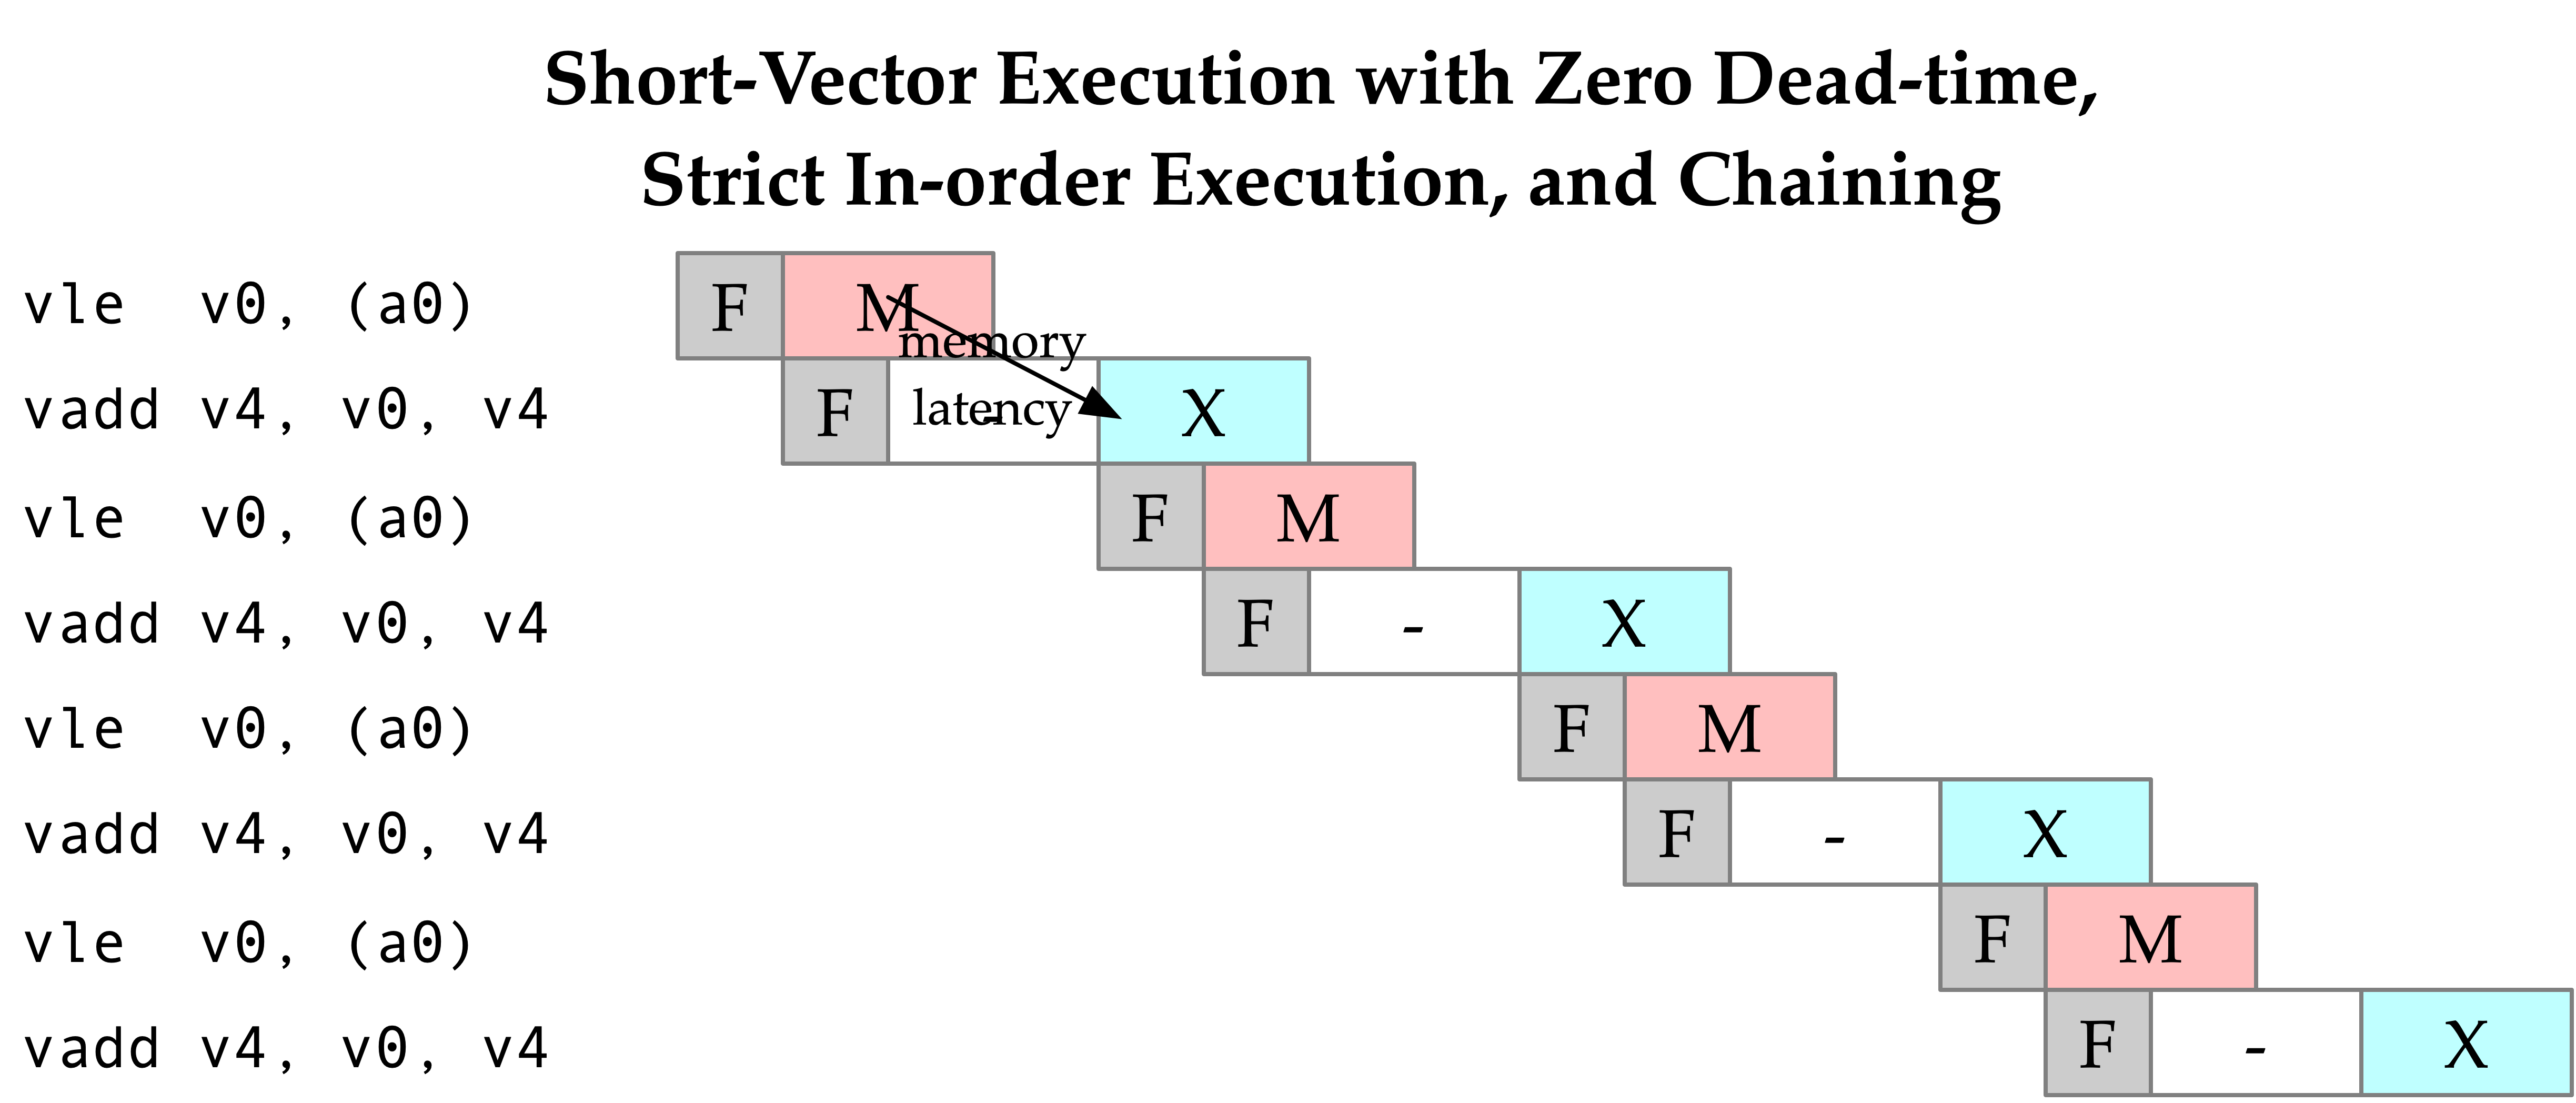
\includegraphics[scale=0.45]{short-vectors-in-order.png}
  \caption{Pipeline diagram of instruction execution with short vector lengths, zero-cycle dead time, strict in-order execution, and chaining. Instructions in the X and M pipelines must begin execution in-order.}
  \label{fig:short-inorder}
\end{figure}

Figure \ref{fig:short-inorder} highlights the importance of limited out-of-order execution for short-vector microarchitectures like Saturn.
Unlike in Figure \ref{fig:short}, the machine in this example requires the instructions to enter the datapath in-order.
Requiring strict in-order execution would substantially degrade performance for suboptimally scheduled vector code.
Despite the same zero-cycle dead time, the restriction on in-order execution prevents the machine from aggressively issuing instructions to hide the latency in the M pipe.

\subsubsection{Compared to Long-Vector Units}

Long-vector microarchitectures feature very-long-vector-lengths distributed across many parallel vector lanes.
Such implementations typically store their vector register files in dense lane-distributed SRAM banks.

Given the very long vector lengths, vector instructions are executed in a deeply temporal manner, even across many parallel vector lanes.
Thus, instruction throughput is less critical for maintaining high utilization of functional units.
Instead, long-vector microarchitectures typically derive efficiency and high utilization by amortizing overheads over fewer long-chime inflight instructions.

\begin{figure}[h]
  \centering
  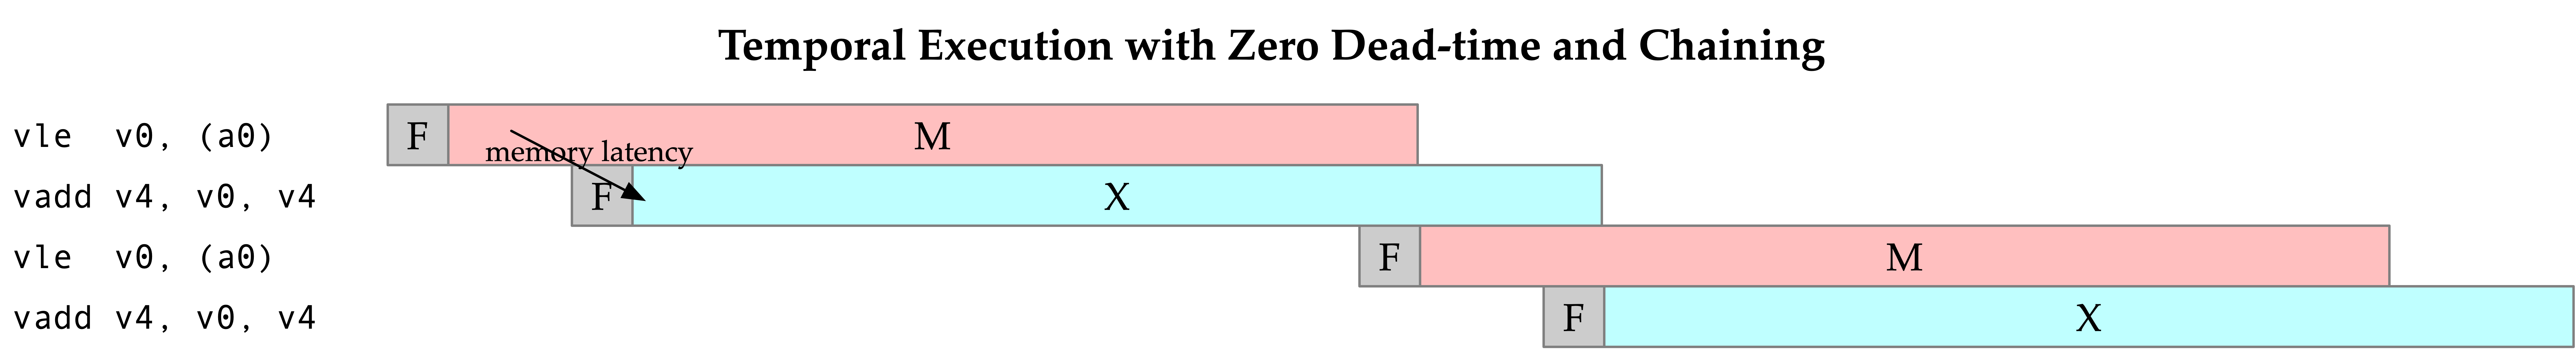
\includegraphics[scale=0.38]{long-vectors.png}
  \caption{Pipeline diagram of instruction execution in a deeply-temporal long-vector machine with zero dead time.}
  \label{fig:long}
\end{figure}

Figure \ref{fig:long} shows an example pipeline diagram of a vector loop in a deeply temporal long-vector machine.
Unlike in the short-vector example in Figure \ref{fig:short}, Instruction throughput requirements are minimal and strict in-order execution is sufficient for maintaining high utilization of the datapaths.

\begin{figure}[h]
  \centering
  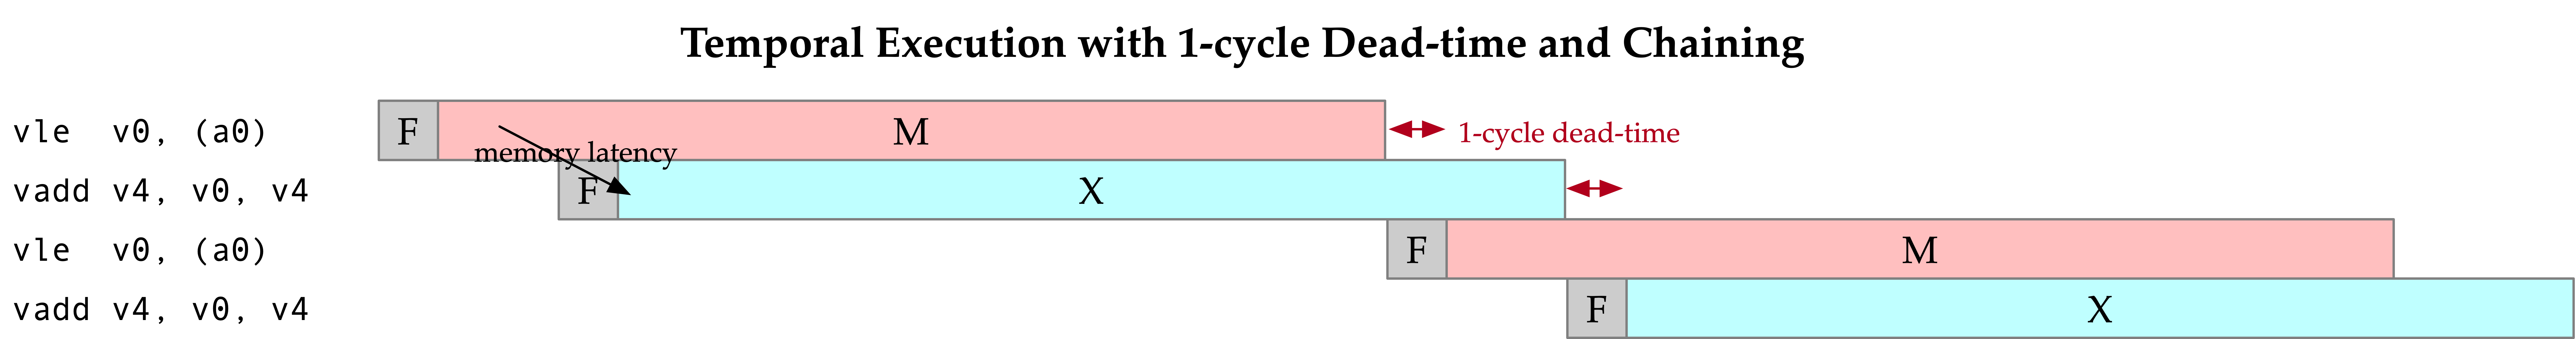
\includegraphics[scale=0.38]{long-vectors-dead.png}
  \caption{Pipeline diagram of instruction execution in a deeply-temporal long-vector machine with 1-cycle dead time.}
  \label{fig:long-dead}
\end{figure}

Figure \ref{fig:long-dead} highlights how dead time in a deeply-temporal vector-unit is amortized over many cycles of temporal execution per instruction.
This contrasts with the Saturn-like short-vector machine, in which short chimes cannot hide dead time.

For DSP deployments, the long-vectors paradigm is particularly ill-suited when compared to short-vectors Saturn-like cores.

\begin{itemize}
\item Many DSP applications feature short and/or widely varying application vector lengths. This makes it difficult for long-vector machines to effectively utilize their resources as it precludes deep temporal execution. Short-vector machines can achieve higher utilization on these shorter application vector lengths.
\item Short-vector machines use an inherently lower capacity vector register file, which has positive implications in terms of silicon area and power consumption.
\item Short-vector machines can still reduce IPC requirements and dynamic instruction counts on applications with long vector lengths by leveraging the register grouping capabilities of modern vector ISAs.
\end{itemize}

\subsubsection{Compared to General-purpose SIMD Cores}

SIMD datapaths in general-purpose cores are typically deeply integrated into the scalar instruction execution pipeline.
In these designs, existing capabilities for out-of-order execution, speculative execution, superscalar fetch, and register renaming are leveraged to maximize SIMD datapath utilization.
While these features are costly in power and area, they are fundamental necessary components of modern general-purpose cores, and thus are also leveraged when executing SIMD code.

\begin{figure}[h]
  \centering
  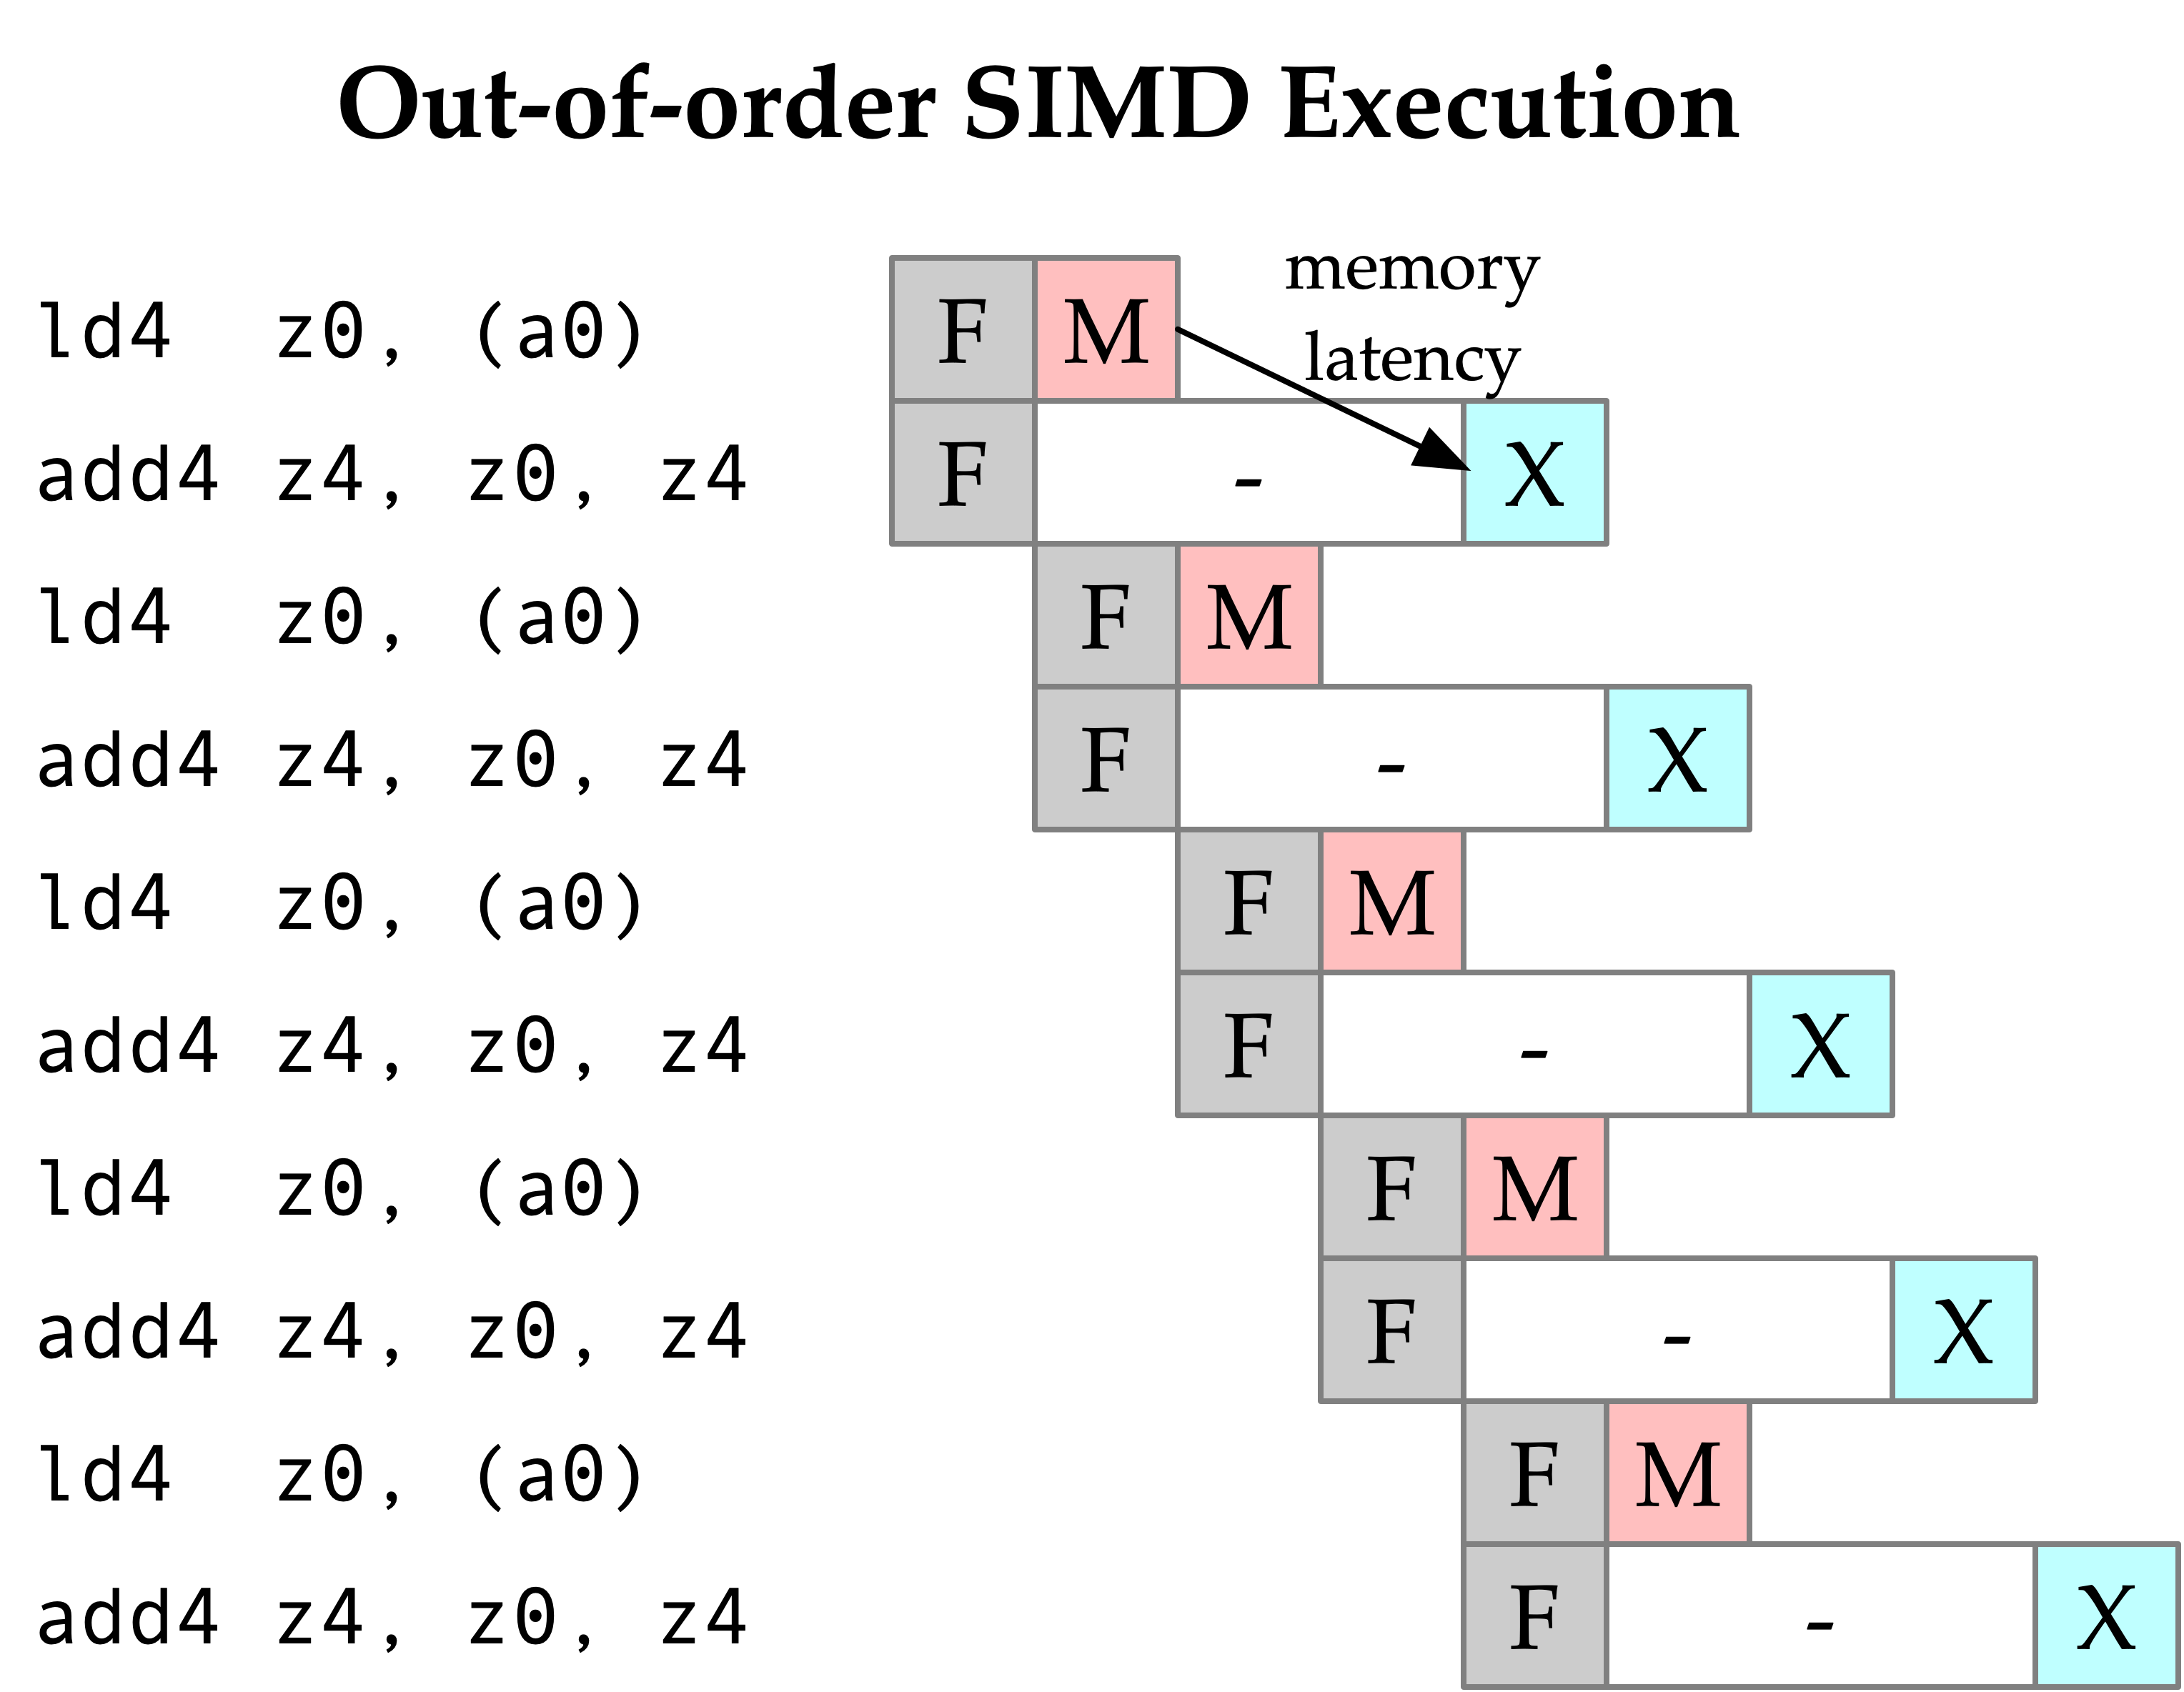
\includegraphics[scale=0.45]{ooo-simd.png}
  \caption{Pipeline diagram of instruction execution in an out-of-order SIMD machine.}
  \label{fig:ooo}
\end{figure}

Figure \ref{fig:ooo} depicts an example pipeline diagram of a SIMD loop in an out-of-order core with SIMD extensions.
Notably, as these machines are typically designed with single-chime instruction execution, high instruction throughput is necessary to maintain high utilization of multiple datapaths.
Furthermore, register renaming is required to enable execution past the WAW and WAR hazards in this example loop.

Unlike these cores, a Saturn-like short-vector design does not rely on costly features like high-throughput instruction fetch, out-of-order execution, speculative execution, or register-renaming.
Efficient scheduling of short-chime vector instructions with a limited capability for out-of-order execution is sufficient for maintaining datapath utilization on memory workloads, even with a minimal in-order scalar core.

\subsubsection{Compared to VLIW + SIMD DSP Cores}

VLIW cores with SIMD extensions also rely on high-throughput instruction fetch for performance through VLIW instruction encodings.
VLIW instructions enable low-cost, low-complexity superscalar fetch and provide the programmer with precise control over instruction scheduling.

\begin{figure}[h]
  \centering
  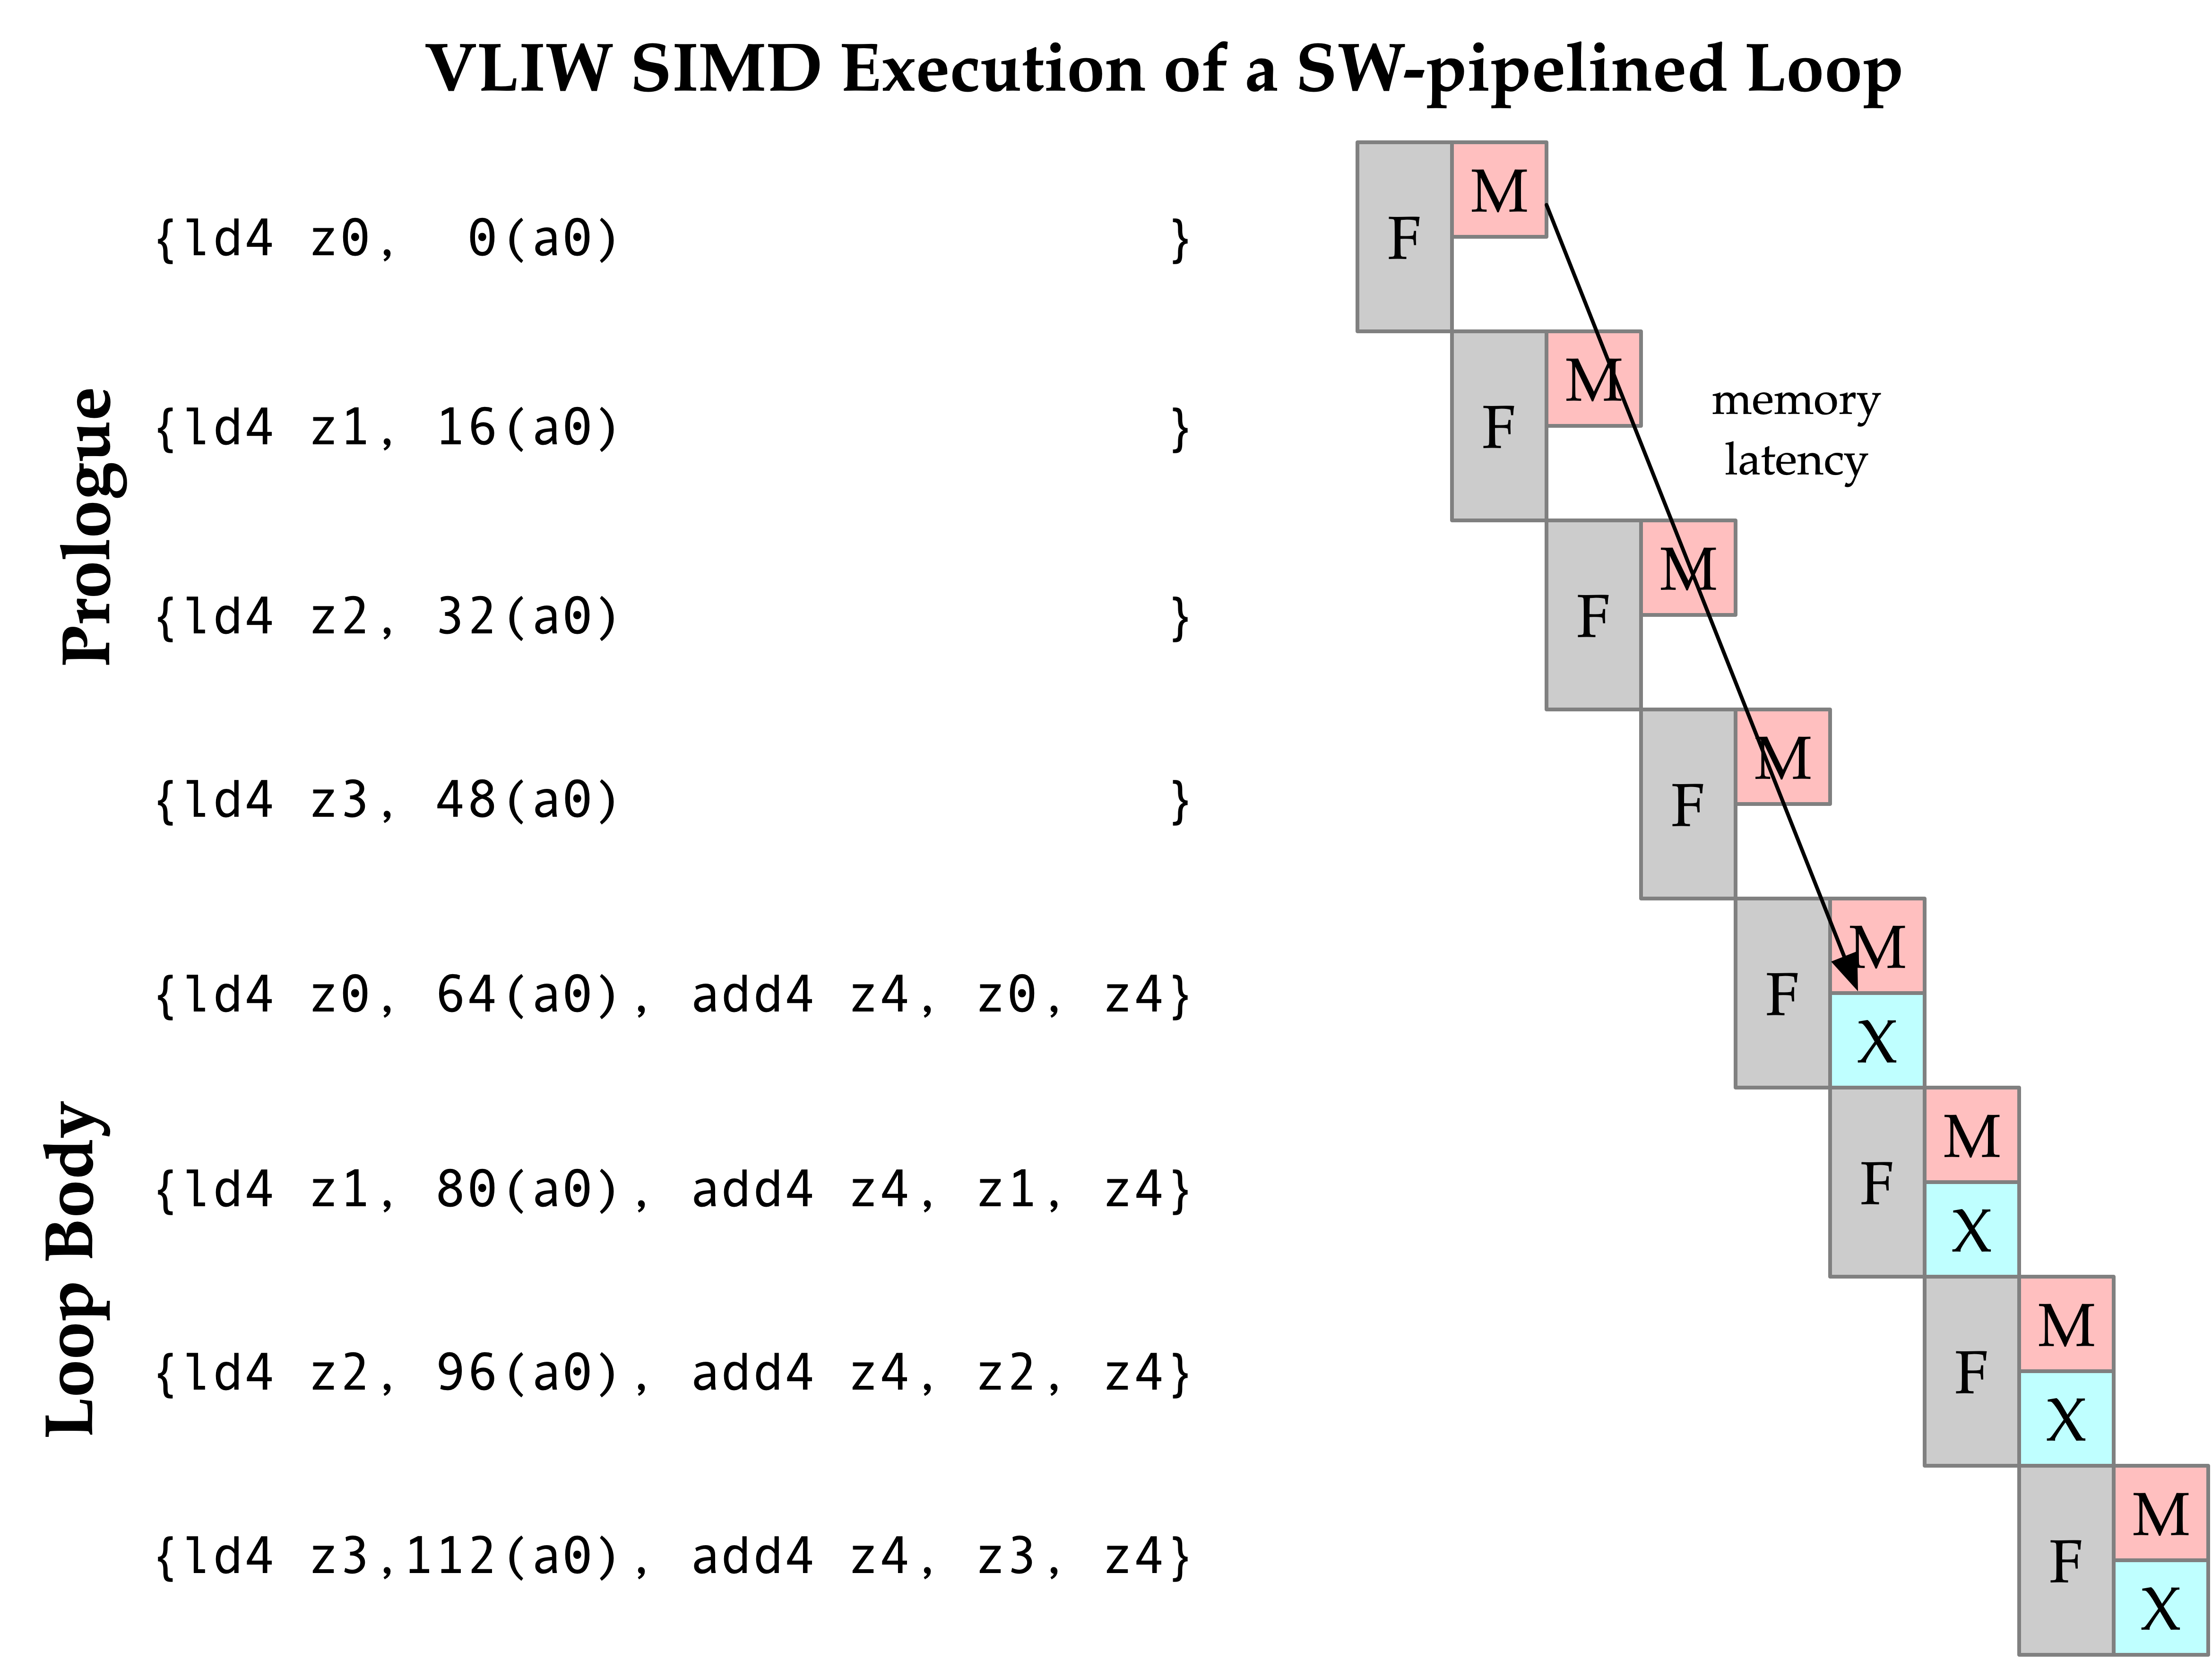
\includegraphics[scale=0.45]{vliw-simd.png}
  \caption{Pipeline diagram of instruction execution in a VLIW SIMD machine, executing a software-pipelined loop.}
  \label{fig:vliw}
\end{figure}

Figure \ref{fig:vliw} depicts an example software-pipelined loop executing on a VLIW-SIMD machine.
While VLIW instruction encodings effectively provide high operation throughput to the datapath, leveraging them typically requires precisely optimized static scheduling, such as with extensive loop unrolling and software-pipelining.
Notably, the verbose prologue and epilogue sections of such loops inflate the code size beyond what a normal vector or scalar loop would require.

Unlike SIMD datapaths in VLIW cores, a Saturn-like short-vector design does not require the high instruction throughput of VLIW fetch.
A short-vector machine's more aggressive capability for dynamic instruction scheduling also diminishes the need for precisely scheduled microarchitecture-aware code, compared to VLIW-SIMD designs.
